
% Default to the notebook output style

    


% Inherit from the specified cell style.




    
\documentclass[11pt]{article}

    
    
    \usepackage[T1]{fontenc}
    % Nicer default font (+ math font) than Computer Modern for most use cases
    \usepackage{mathpazo}

    % Basic figure setup, for now with no caption control since it's done
    % automatically by Pandoc (which extracts ![](path) syntax from Markdown).
    \usepackage{graphicx}
    % We will generate all images so they have a width \maxwidth. This means
    % that they will get their normal width if they fit onto the page, but
    % are scaled down if they would overflow the margins.
    \makeatletter
    \def\maxwidth{\ifdim\Gin@nat@width>\linewidth\linewidth
    \else\Gin@nat@width\fi}
    \makeatother
    \let\Oldincludegraphics\includegraphics
    % Set max figure width to be 80% of text width, for now hardcoded.
    \renewcommand{\includegraphics}[1]{\Oldincludegraphics[width=.8\maxwidth]{#1}}
    % Ensure that by default, figures have no caption (until we provide a
    % proper Figure object with a Caption API and a way to capture that
    % in the conversion process - todo).
    \usepackage{caption}
    \DeclareCaptionLabelFormat{nolabel}{}
    \captionsetup{labelformat=nolabel}

    \usepackage{adjustbox} % Used to constrain images to a maximum size 
    \usepackage{xcolor} % Allow colors to be defined
    \usepackage{enumerate} % Needed for markdown enumerations to work
    \usepackage{geometry} % Used to adjust the document margins
    \usepackage{amsmath} % Equations
    \usepackage{amssymb} % Equations
    \usepackage{textcomp} % defines textquotesingle
    % Hack from http://tex.stackexchange.com/a/47451/13684:
    \AtBeginDocument{%
        \def\PYZsq{\textquotesingle}% Upright quotes in Pygmentized code
    }
    \usepackage{upquote} % Upright quotes for verbatim code
    \usepackage{eurosym} % defines \euro
    \usepackage[mathletters]{ucs} % Extended unicode (utf-8) support
    \usepackage[utf8x]{inputenc} % Allow utf-8 characters in the tex document
    \usepackage{fancyvrb} % verbatim replacement that allows latex
    \usepackage{grffile} % extends the file name processing of package graphics 
                         % to support a larger range 
    % The hyperref package gives us a pdf with properly built
    % internal navigation ('pdf bookmarks' for the table of contents,
    % internal cross-reference links, web links for URLs, etc.)
    \usepackage{hyperref}
    \usepackage{longtable} % longtable support required by pandoc >1.10
    \usepackage{booktabs}  % table support for pandoc > 1.12.2
    \usepackage[inline]{enumitem} % IRkernel/repr support (it uses the enumerate* environment)
    \usepackage[normalem]{ulem} % ulem is needed to support strikethroughs (\sout)
                                % normalem makes italics be italics, not underlines
    

    
    
    % Colors for the hyperref package
    \definecolor{urlcolor}{rgb}{0,.145,.698}
    \definecolor{linkcolor}{rgb}{.71,0.21,0.01}
    \definecolor{citecolor}{rgb}{.12,.54,.11}

    % ANSI colors
    \definecolor{ansi-black}{HTML}{3E424D}
    \definecolor{ansi-black-intense}{HTML}{282C36}
    \definecolor{ansi-red}{HTML}{E75C58}
    \definecolor{ansi-red-intense}{HTML}{B22B31}
    \definecolor{ansi-green}{HTML}{00A250}
    \definecolor{ansi-green-intense}{HTML}{007427}
    \definecolor{ansi-yellow}{HTML}{DDB62B}
    \definecolor{ansi-yellow-intense}{HTML}{B27D12}
    \definecolor{ansi-blue}{HTML}{208FFB}
    \definecolor{ansi-blue-intense}{HTML}{0065CA}
    \definecolor{ansi-magenta}{HTML}{D160C4}
    \definecolor{ansi-magenta-intense}{HTML}{A03196}
    \definecolor{ansi-cyan}{HTML}{60C6C8}
    \definecolor{ansi-cyan-intense}{HTML}{258F8F}
    \definecolor{ansi-white}{HTML}{C5C1B4}
    \definecolor{ansi-white-intense}{HTML}{A1A6B2}

    % commands and environments needed by pandoc snippets
    % extracted from the output of `pandoc -s`
    \providecommand{\tightlist}{%
      \setlength{\itemsep}{0pt}\setlength{\parskip}{0pt}}
    \DefineVerbatimEnvironment{Highlighting}{Verbatim}{commandchars=\\\{\}}
    % Add ',fontsize=\small' for more characters per line
    \newenvironment{Shaded}{}{}
    \newcommand{\KeywordTok}[1]{\textcolor[rgb]{0.00,0.44,0.13}{\textbf{{#1}}}}
    \newcommand{\DataTypeTok}[1]{\textcolor[rgb]{0.56,0.13,0.00}{{#1}}}
    \newcommand{\DecValTok}[1]{\textcolor[rgb]{0.25,0.63,0.44}{{#1}}}
    \newcommand{\BaseNTok}[1]{\textcolor[rgb]{0.25,0.63,0.44}{{#1}}}
    \newcommand{\FloatTok}[1]{\textcolor[rgb]{0.25,0.63,0.44}{{#1}}}
    \newcommand{\CharTok}[1]{\textcolor[rgb]{0.25,0.44,0.63}{{#1}}}
    \newcommand{\StringTok}[1]{\textcolor[rgb]{0.25,0.44,0.63}{{#1}}}
    \newcommand{\CommentTok}[1]{\textcolor[rgb]{0.38,0.63,0.69}{\textit{{#1}}}}
    \newcommand{\OtherTok}[1]{\textcolor[rgb]{0.00,0.44,0.13}{{#1}}}
    \newcommand{\AlertTok}[1]{\textcolor[rgb]{1.00,0.00,0.00}{\textbf{{#1}}}}
    \newcommand{\FunctionTok}[1]{\textcolor[rgb]{0.02,0.16,0.49}{{#1}}}
    \newcommand{\RegionMarkerTok}[1]{{#1}}
    \newcommand{\ErrorTok}[1]{\textcolor[rgb]{1.00,0.00,0.00}{\textbf{{#1}}}}
    \newcommand{\NormalTok}[1]{{#1}}
    
    % Additional commands for more recent versions of Pandoc
    \newcommand{\ConstantTok}[1]{\textcolor[rgb]{0.53,0.00,0.00}{{#1}}}
    \newcommand{\SpecialCharTok}[1]{\textcolor[rgb]{0.25,0.44,0.63}{{#1}}}
    \newcommand{\VerbatimStringTok}[1]{\textcolor[rgb]{0.25,0.44,0.63}{{#1}}}
    \newcommand{\SpecialStringTok}[1]{\textcolor[rgb]{0.73,0.40,0.53}{{#1}}}
    \newcommand{\ImportTok}[1]{{#1}}
    \newcommand{\DocumentationTok}[1]{\textcolor[rgb]{0.73,0.13,0.13}{\textit{{#1}}}}
    \newcommand{\AnnotationTok}[1]{\textcolor[rgb]{0.38,0.63,0.69}{\textbf{\textit{{#1}}}}}
    \newcommand{\CommentVarTok}[1]{\textcolor[rgb]{0.38,0.63,0.69}{\textbf{\textit{{#1}}}}}
    \newcommand{\VariableTok}[1]{\textcolor[rgb]{0.10,0.09,0.49}{{#1}}}
    \newcommand{\ControlFlowTok}[1]{\textcolor[rgb]{0.00,0.44,0.13}{\textbf{{#1}}}}
    \newcommand{\OperatorTok}[1]{\textcolor[rgb]{0.40,0.40,0.40}{{#1}}}
    \newcommand{\BuiltInTok}[1]{{#1}}
    \newcommand{\ExtensionTok}[1]{{#1}}
    \newcommand{\PreprocessorTok}[1]{\textcolor[rgb]{0.74,0.48,0.00}{{#1}}}
    \newcommand{\AttributeTok}[1]{\textcolor[rgb]{0.49,0.56,0.16}{{#1}}}
    \newcommand{\InformationTok}[1]{\textcolor[rgb]{0.38,0.63,0.69}{\textbf{\textit{{#1}}}}}
    \newcommand{\WarningTok}[1]{\textcolor[rgb]{0.38,0.63,0.69}{\textbf{\textit{{#1}}}}}
    
    
    % Define a nice break command that doesn't care if a line doesn't already
    % exist.
    \def\br{\hspace*{\fill} \\* }
    % Math Jax compatability definitions
    \def\gt{>}
    \def\lt{<}
    % Document parameters
    \title{Clase 01 - Introducci?n al Aprendizaje de M?quina}
    
    
    

    % Pygments definitions
    
\makeatletter
\def\PY@reset{\let\PY@it=\relax \let\PY@bf=\relax%
    \let\PY@ul=\relax \let\PY@tc=\relax%
    \let\PY@bc=\relax \let\PY@ff=\relax}
\def\PY@tok#1{\csname PY@tok@#1\endcsname}
\def\PY@toks#1+{\ifx\relax#1\empty\else%
    \PY@tok{#1}\expandafter\PY@toks\fi}
\def\PY@do#1{\PY@bc{\PY@tc{\PY@ul{%
    \PY@it{\PY@bf{\PY@ff{#1}}}}}}}
\def\PY#1#2{\PY@reset\PY@toks#1+\relax+\PY@do{#2}}

\expandafter\def\csname PY@tok@gd\endcsname{\def\PY@tc##1{\textcolor[rgb]{0.63,0.00,0.00}{##1}}}
\expandafter\def\csname PY@tok@gu\endcsname{\let\PY@bf=\textbf\def\PY@tc##1{\textcolor[rgb]{0.50,0.00,0.50}{##1}}}
\expandafter\def\csname PY@tok@gt\endcsname{\def\PY@tc##1{\textcolor[rgb]{0.00,0.27,0.87}{##1}}}
\expandafter\def\csname PY@tok@gs\endcsname{\let\PY@bf=\textbf}
\expandafter\def\csname PY@tok@gr\endcsname{\def\PY@tc##1{\textcolor[rgb]{1.00,0.00,0.00}{##1}}}
\expandafter\def\csname PY@tok@cm\endcsname{\let\PY@it=\textit\def\PY@tc##1{\textcolor[rgb]{0.25,0.50,0.50}{##1}}}
\expandafter\def\csname PY@tok@vg\endcsname{\def\PY@tc##1{\textcolor[rgb]{0.10,0.09,0.49}{##1}}}
\expandafter\def\csname PY@tok@vi\endcsname{\def\PY@tc##1{\textcolor[rgb]{0.10,0.09,0.49}{##1}}}
\expandafter\def\csname PY@tok@vm\endcsname{\def\PY@tc##1{\textcolor[rgb]{0.10,0.09,0.49}{##1}}}
\expandafter\def\csname PY@tok@mh\endcsname{\def\PY@tc##1{\textcolor[rgb]{0.40,0.40,0.40}{##1}}}
\expandafter\def\csname PY@tok@cs\endcsname{\let\PY@it=\textit\def\PY@tc##1{\textcolor[rgb]{0.25,0.50,0.50}{##1}}}
\expandafter\def\csname PY@tok@ge\endcsname{\let\PY@it=\textit}
\expandafter\def\csname PY@tok@vc\endcsname{\def\PY@tc##1{\textcolor[rgb]{0.10,0.09,0.49}{##1}}}
\expandafter\def\csname PY@tok@il\endcsname{\def\PY@tc##1{\textcolor[rgb]{0.40,0.40,0.40}{##1}}}
\expandafter\def\csname PY@tok@go\endcsname{\def\PY@tc##1{\textcolor[rgb]{0.53,0.53,0.53}{##1}}}
\expandafter\def\csname PY@tok@cp\endcsname{\def\PY@tc##1{\textcolor[rgb]{0.74,0.48,0.00}{##1}}}
\expandafter\def\csname PY@tok@gi\endcsname{\def\PY@tc##1{\textcolor[rgb]{0.00,0.63,0.00}{##1}}}
\expandafter\def\csname PY@tok@gh\endcsname{\let\PY@bf=\textbf\def\PY@tc##1{\textcolor[rgb]{0.00,0.00,0.50}{##1}}}
\expandafter\def\csname PY@tok@ni\endcsname{\let\PY@bf=\textbf\def\PY@tc##1{\textcolor[rgb]{0.60,0.60,0.60}{##1}}}
\expandafter\def\csname PY@tok@nl\endcsname{\def\PY@tc##1{\textcolor[rgb]{0.63,0.63,0.00}{##1}}}
\expandafter\def\csname PY@tok@nn\endcsname{\let\PY@bf=\textbf\def\PY@tc##1{\textcolor[rgb]{0.00,0.00,1.00}{##1}}}
\expandafter\def\csname PY@tok@no\endcsname{\def\PY@tc##1{\textcolor[rgb]{0.53,0.00,0.00}{##1}}}
\expandafter\def\csname PY@tok@na\endcsname{\def\PY@tc##1{\textcolor[rgb]{0.49,0.56,0.16}{##1}}}
\expandafter\def\csname PY@tok@nb\endcsname{\def\PY@tc##1{\textcolor[rgb]{0.00,0.50,0.00}{##1}}}
\expandafter\def\csname PY@tok@nc\endcsname{\let\PY@bf=\textbf\def\PY@tc##1{\textcolor[rgb]{0.00,0.00,1.00}{##1}}}
\expandafter\def\csname PY@tok@nd\endcsname{\def\PY@tc##1{\textcolor[rgb]{0.67,0.13,1.00}{##1}}}
\expandafter\def\csname PY@tok@ne\endcsname{\let\PY@bf=\textbf\def\PY@tc##1{\textcolor[rgb]{0.82,0.25,0.23}{##1}}}
\expandafter\def\csname PY@tok@nf\endcsname{\def\PY@tc##1{\textcolor[rgb]{0.00,0.00,1.00}{##1}}}
\expandafter\def\csname PY@tok@si\endcsname{\let\PY@bf=\textbf\def\PY@tc##1{\textcolor[rgb]{0.73,0.40,0.53}{##1}}}
\expandafter\def\csname PY@tok@s2\endcsname{\def\PY@tc##1{\textcolor[rgb]{0.73,0.13,0.13}{##1}}}
\expandafter\def\csname PY@tok@nt\endcsname{\let\PY@bf=\textbf\def\PY@tc##1{\textcolor[rgb]{0.00,0.50,0.00}{##1}}}
\expandafter\def\csname PY@tok@nv\endcsname{\def\PY@tc##1{\textcolor[rgb]{0.10,0.09,0.49}{##1}}}
\expandafter\def\csname PY@tok@s1\endcsname{\def\PY@tc##1{\textcolor[rgb]{0.73,0.13,0.13}{##1}}}
\expandafter\def\csname PY@tok@dl\endcsname{\def\PY@tc##1{\textcolor[rgb]{0.73,0.13,0.13}{##1}}}
\expandafter\def\csname PY@tok@ch\endcsname{\let\PY@it=\textit\def\PY@tc##1{\textcolor[rgb]{0.25,0.50,0.50}{##1}}}
\expandafter\def\csname PY@tok@m\endcsname{\def\PY@tc##1{\textcolor[rgb]{0.40,0.40,0.40}{##1}}}
\expandafter\def\csname PY@tok@gp\endcsname{\let\PY@bf=\textbf\def\PY@tc##1{\textcolor[rgb]{0.00,0.00,0.50}{##1}}}
\expandafter\def\csname PY@tok@sh\endcsname{\def\PY@tc##1{\textcolor[rgb]{0.73,0.13,0.13}{##1}}}
\expandafter\def\csname PY@tok@ow\endcsname{\let\PY@bf=\textbf\def\PY@tc##1{\textcolor[rgb]{0.67,0.13,1.00}{##1}}}
\expandafter\def\csname PY@tok@sx\endcsname{\def\PY@tc##1{\textcolor[rgb]{0.00,0.50,0.00}{##1}}}
\expandafter\def\csname PY@tok@bp\endcsname{\def\PY@tc##1{\textcolor[rgb]{0.00,0.50,0.00}{##1}}}
\expandafter\def\csname PY@tok@c1\endcsname{\let\PY@it=\textit\def\PY@tc##1{\textcolor[rgb]{0.25,0.50,0.50}{##1}}}
\expandafter\def\csname PY@tok@fm\endcsname{\def\PY@tc##1{\textcolor[rgb]{0.00,0.00,1.00}{##1}}}
\expandafter\def\csname PY@tok@o\endcsname{\def\PY@tc##1{\textcolor[rgb]{0.40,0.40,0.40}{##1}}}
\expandafter\def\csname PY@tok@kc\endcsname{\let\PY@bf=\textbf\def\PY@tc##1{\textcolor[rgb]{0.00,0.50,0.00}{##1}}}
\expandafter\def\csname PY@tok@c\endcsname{\let\PY@it=\textit\def\PY@tc##1{\textcolor[rgb]{0.25,0.50,0.50}{##1}}}
\expandafter\def\csname PY@tok@mf\endcsname{\def\PY@tc##1{\textcolor[rgb]{0.40,0.40,0.40}{##1}}}
\expandafter\def\csname PY@tok@err\endcsname{\def\PY@bc##1{\setlength{\fboxsep}{0pt}\fcolorbox[rgb]{1.00,0.00,0.00}{1,1,1}{\strut ##1}}}
\expandafter\def\csname PY@tok@mb\endcsname{\def\PY@tc##1{\textcolor[rgb]{0.40,0.40,0.40}{##1}}}
\expandafter\def\csname PY@tok@ss\endcsname{\def\PY@tc##1{\textcolor[rgb]{0.10,0.09,0.49}{##1}}}
\expandafter\def\csname PY@tok@sr\endcsname{\def\PY@tc##1{\textcolor[rgb]{0.73,0.40,0.53}{##1}}}
\expandafter\def\csname PY@tok@mo\endcsname{\def\PY@tc##1{\textcolor[rgb]{0.40,0.40,0.40}{##1}}}
\expandafter\def\csname PY@tok@kd\endcsname{\let\PY@bf=\textbf\def\PY@tc##1{\textcolor[rgb]{0.00,0.50,0.00}{##1}}}
\expandafter\def\csname PY@tok@mi\endcsname{\def\PY@tc##1{\textcolor[rgb]{0.40,0.40,0.40}{##1}}}
\expandafter\def\csname PY@tok@kn\endcsname{\let\PY@bf=\textbf\def\PY@tc##1{\textcolor[rgb]{0.00,0.50,0.00}{##1}}}
\expandafter\def\csname PY@tok@cpf\endcsname{\let\PY@it=\textit\def\PY@tc##1{\textcolor[rgb]{0.25,0.50,0.50}{##1}}}
\expandafter\def\csname PY@tok@kr\endcsname{\let\PY@bf=\textbf\def\PY@tc##1{\textcolor[rgb]{0.00,0.50,0.00}{##1}}}
\expandafter\def\csname PY@tok@s\endcsname{\def\PY@tc##1{\textcolor[rgb]{0.73,0.13,0.13}{##1}}}
\expandafter\def\csname PY@tok@kp\endcsname{\def\PY@tc##1{\textcolor[rgb]{0.00,0.50,0.00}{##1}}}
\expandafter\def\csname PY@tok@w\endcsname{\def\PY@tc##1{\textcolor[rgb]{0.73,0.73,0.73}{##1}}}
\expandafter\def\csname PY@tok@kt\endcsname{\def\PY@tc##1{\textcolor[rgb]{0.69,0.00,0.25}{##1}}}
\expandafter\def\csname PY@tok@sc\endcsname{\def\PY@tc##1{\textcolor[rgb]{0.73,0.13,0.13}{##1}}}
\expandafter\def\csname PY@tok@sb\endcsname{\def\PY@tc##1{\textcolor[rgb]{0.73,0.13,0.13}{##1}}}
\expandafter\def\csname PY@tok@sa\endcsname{\def\PY@tc##1{\textcolor[rgb]{0.73,0.13,0.13}{##1}}}
\expandafter\def\csname PY@tok@k\endcsname{\let\PY@bf=\textbf\def\PY@tc##1{\textcolor[rgb]{0.00,0.50,0.00}{##1}}}
\expandafter\def\csname PY@tok@se\endcsname{\let\PY@bf=\textbf\def\PY@tc##1{\textcolor[rgb]{0.73,0.40,0.13}{##1}}}
\expandafter\def\csname PY@tok@sd\endcsname{\let\PY@it=\textit\def\PY@tc##1{\textcolor[rgb]{0.73,0.13,0.13}{##1}}}

\def\PYZbs{\char`\\}
\def\PYZus{\char`\_}
\def\PYZob{\char`\{}
\def\PYZcb{\char`\}}
\def\PYZca{\char`\^}
\def\PYZam{\char`\&}
\def\PYZlt{\char`\<}
\def\PYZgt{\char`\>}
\def\PYZsh{\char`\#}
\def\PYZpc{\char`\%}
\def\PYZdl{\char`\$}
\def\PYZhy{\char`\-}
\def\PYZsq{\char`\'}
\def\PYZdq{\char`\"}
\def\PYZti{\char`\~}
% for compatibility with earlier versions
\def\PYZat{@}
\def\PYZlb{[}
\def\PYZrb{]}
\makeatother


    % Exact colors from NB
    \definecolor{incolor}{rgb}{0.0, 0.0, 0.5}
    \definecolor{outcolor}{rgb}{0.545, 0.0, 0.0}



    
    % Prevent overflowing lines due to hard-to-break entities
    \sloppy 
    % Setup hyperref package
    \hypersetup{
      breaklinks=true,  % so long urls are correctly broken across lines
      colorlinks=true,
      urlcolor=urlcolor,
      linkcolor=linkcolor,
      citecolor=citecolor,
      }
    % Slightly bigger margins than the latex defaults
    
    \geometry{verbose,tmargin=1in,bmargin=1in,lmargin=1in,rmargin=1in}
    
    

    \begin{document}
    
    
    \maketitle
    
    

    
    \section{\texorpdfstring{\textbf{Introducción al aprendizaje de
máquina}}{Introducción al aprendizaje de máquina}}\label{introducciuxf3n-al-aprendizaje-de-muxe1quina}

    \subsection{** Julián D. Arias
Londoño**}\label{juliuxe1n-d.-arias-londouxf1o}

    Profesor Asistente Departamento de Ingeniería de Sistemas Universidad de
Antioquia, Medellín, Colombia jdarias@udea.edu.co

    \begin{Verbatim}[commandchars=\\\{\}]
{\color{incolor}In [{\color{incolor}1}]:} \PY{c+c1}{\PYZsh{}\PYZsh{} Bibliotecas}
        \PY{c+c1}{\PYZsh{} Sirve para mostrar las graficas generadas por matplotlib inmediatemente despues de que sea llamada.}
        \PY{o}{\PYZpc{}}\PY{k}{matplotlib} inline 
        \PY{k+kn}{from} \PY{n+nn}{IPython.display} \PY{k+kn}{import} \PY{n}{Image}
        
        \PY{c+c1}{\PYZsh{}Numpy es una biblioteca que nos permite muy buen soporte a las operaciones entre matrices y vectores}
        \PY{k+kn}{import} \PY{n+nn}{numpy} \PY{k+kn}{as} \PY{n+nn}{np}
        
        \PY{c+c1}{\PYZsh{} Biblioteca usada para diseñar y mostrar graficos.}
        \PY{k+kn}{import} \PY{n+nn}{matplotlib.pyplot} \PY{k+kn}{as} \PY{n+nn}{plt} 
        \PY{k+kn}{import} \PY{n+nn}{seaborn} \PY{k+kn}{as} \PY{n+nn}{sns}
        \PY{n}{sns}\PY{o}{.}\PY{n}{set}\PY{p}{(}\PY{n}{color\PYZus{}codes}\PY{o}{=}\PY{n+nb+bp}{True}\PY{p}{)}
        
        \PY{c+c1}{\PYZsh{} Biblioteca con algoritmos de Machine Learning ya implementados}
        \PY{k+kn}{from} \PY{n+nn}{sklearn} \PY{k+kn}{import} \PY{n}{datasets}  \PY{c+c1}{\PYZsh{} Se importa el modulo de bases de datos de sklearn }
\end{Verbatim}

    \subsubsection{** Definición**}\label{definiciuxf3n}

El aprendizaje de máquina (En inglés: Machine Learning (ML)) es una rama
de la inteligencia artifical enfocada al estudio de sistemas que pueden
"\emph{aprender}" a partir de datos. De acuerdo con {[}1{]}, ML son un
conjunto de métodos que pueden detectar automáticamente patrones en un
conjunto de datos, aprenderlos y luego usarlos para predicir datos
futuros o realizar otro tipo de decisiones bajo incertidumbre.

    Ejemplos de aplicaciones de ML:

    \begin{itemize}
\tightlist
\item
  Reconocimiento de Caracteres escritos a mano
\end{itemize}

    \begin{figure}[htbp]
\centering
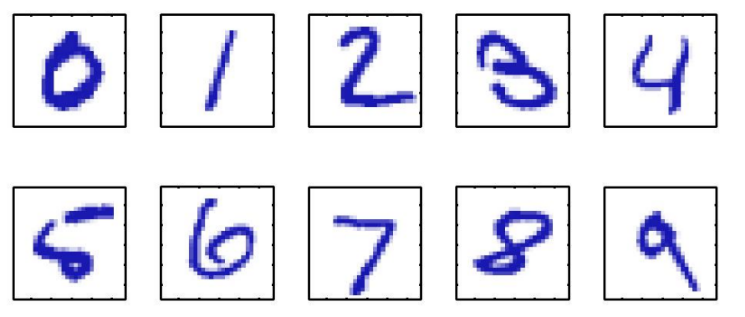
\includegraphics{./Images/HR.png}
\caption{alt text}
\end{figure}

    \begin{itemize}
\tightlist
\item
  Reconocimiento de Rostros
\end{itemize}

    \begin{figure}[htbp]
\centering
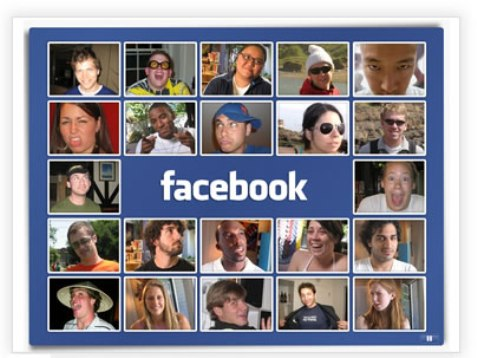
\includegraphics{./Images/facebook-photo.jpeg}
\caption{alt text}
\end{figure}

    \begin{itemize}
\tightlist
\item
  Biometría
\end{itemize}

    \begin{figure}[htbp]
\centering
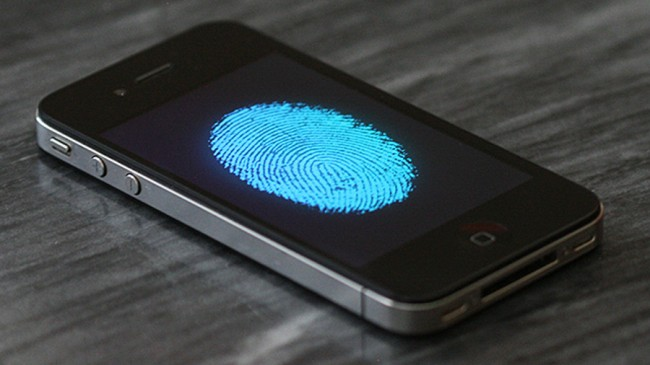
\includegraphics{./Images/iphone-fingerprint.jpeg}
\caption{alt text}
\end{figure}

    Otros ejemplos son:

\begin{enumerate}
\def\labelenumi{\arabic{enumi}.}
\tightlist
\item
  Reconocimiento de Caracteres Ópticos
\item
  Reconocimiento de Tatuajes
\item
  Filtración de Spam
\item
  Reconocimiento de Voz
\item
  Sistemas de Recomendación
\item
  Pronóstico de Variables Económicas
\item
  Diversos Sistemas de Ayuda a la Toma de Decisiones
\end{enumerate}

    Campos relacionados al ML:

\begin{itemize}
\tightlist
\item
  Data Mining
\item
  Information Retrieval
\item
  Knowledge Discovery
\item
  Pattern Recognition
\item
  Probabilistic Methods
\item
  Natural Computing
\item
  Soft Computing
\item
  Multivariate Statistics
\item
  Optimization and Operation Research
\item
  Intelligent Agents and Intelligent Systems
\item
  Parallel Computing
\end{itemize}

    \subsubsection{\texorpdfstring{\textbf{Tipos de Aprendizaje de
Máquina}}{Tipos de Aprendizaje de Máquina}}\label{tipos-de-aprendizaje-de-muxe1quina}

    \paragraph{** Aprendizaje predictivo o supervisado (Supervised
Learning)**}\label{aprendizaje-predictivo-o-supervisado-supervised-learning}

    En el cual el objetivo es aprender un mapeo a partir de entradas
\textbf{x} a salidas y, dado un conjunto de pares entrada-salida
etiquetados
\(\mathit{D} = \left \{ \left ( \mathbf{x}_{i},{y}_{i} \right ) \right \} _{i=1}^{N}\).
En este caso \(\mathit{D}\) se conoce como el \textbf{conjunto de
entrenamiento} y \(\mathit{N}\) es el número de muestras de
entrenamiento.

En una forma simple, cada muestra de entrenamiento \(\mathbf{x}_{i}\) es
un vector de números \(\mathit{d}\)-dimensional que representa variables
o medidas del sistema o fenómeno que se desea modelar y que en el
contexto del aprendizaje de máquinas es común llamarlas **
características** (en inglés ** features **).

    \begin{figure}[htbp]
\centering
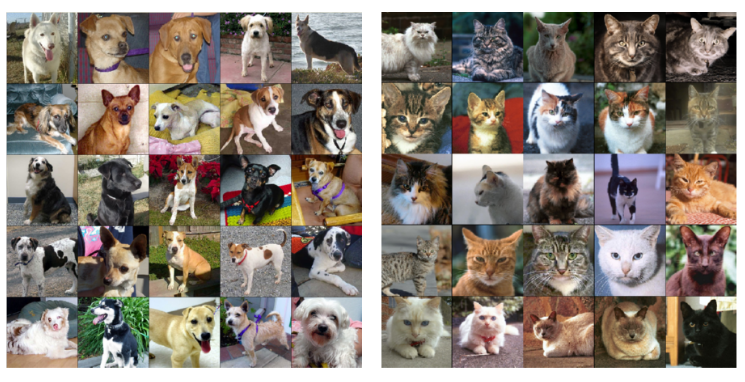
\includegraphics{./Images/Supervised.png}
\caption{alt text}
\end{figure}

    \paragraph{\texorpdfstring{\textbf{Descriptivo o no supervisado
(Unsupervised
Learning)}}{Descriptivo o no supervisado (Unsupervised Learning)}}\label{descriptivo-o-no-supervisado-unsupervised-learning}

    En este caso unicamente se cuenta con un conjunto
\(\mathit{D} = \left \{ \left ( \mathbf{x}_{i} \right ) \right \} _{i=1}^{N}\);
y el objetivo es encontrar "\emph{patrones interesantes} " en los datos.
Algunas veces se le llama ** Descubrimiento de conocimiento.**

    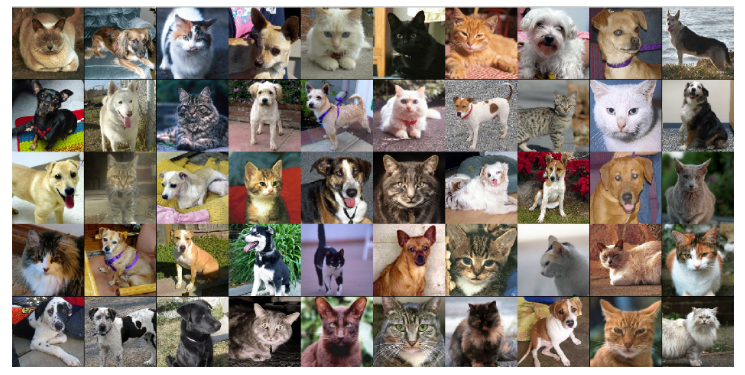
\includegraphics{./Images/Unsupervised.png} ***

    \paragraph{\texorpdfstring{\textbf{Tipos de problemas
supervisados}}{Tipos de problemas supervisados}}\label{tipos-de-problemas-supervisados}

    En general \(\mathbf{x}_{i}\) puede representar un objeto complejo, como
una imagen, una frase, un mensaje de correo electrónico, un cliente, una
serie de tiempo, una cadena de ADN, una molécula, un grafo, etc. En el
aprendizaje supervisado, si la variable de salida yi toma valores
discretos (es categórica), el problema de aprendizaje se conoce como
\textbf{Clasificación}. Si por el contrario yi toma valores reales, el
problema se conoce como \textbf{Regresión}.

    \begin{Verbatim}[commandchars=\\\{\}]
{\color{incolor}In [{\color{incolor}2}]:} \PY{n}{iris} \PY{o}{=} \PY{n}{datasets}\PY{o}{.}\PY{n}{load\PYZus{}iris}\PY{p}{(}\PY{p}{)} \PY{c+c1}{\PYZsh{}  Se carga la base de datos Iris del modulo datasets de sklearn}
        \PY{n}{X}\PY{p}{,} \PY{n}{y} \PY{o}{=} \PY{n}{iris}\PY{o}{.}\PY{n}{data}\PY{p}{,} \PY{n}{iris}\PY{o}{.}\PY{n}{target}
        \PY{c+c1}{\PYZsh{} La variable X contiene las muestras }
        \PY{c+c1}{\PYZsh{} La variable y contiene las etiquetas correspondientes a cada valor de X}
        \PY{n}{plt}\PY{o}{.}\PY{n}{title}\PY{p}{(}\PY{l+s+s1}{\PYZsq{}}\PY{l+s+s1}{Problema de 3 clases}\PY{l+s+s1}{\PYZsq{}}\PY{p}{,} \PY{n}{fontsize}\PY{o}{=}\PY{l+m+mi}{14}\PY{p}{)}
        \PY{n}{plt}\PY{o}{.}\PY{n}{xlabel}\PY{p}{(}\PY{l+s+s1}{\PYZsq{}}\PY{l+s+s1}{Caracteristica 1}\PY{l+s+s1}{\PYZsq{}}\PY{p}{)}
        \PY{n}{plt}\PY{o}{.}\PY{n}{ylabel}\PY{p}{(}\PY{l+s+s1}{\PYZsq{}}\PY{l+s+s1}{Caracteristica 2}\PY{l+s+s1}{\PYZsq{}}\PY{p}{)}
        \PY{n}{plt}\PY{o}{.}\PY{n}{scatter}\PY{p}{(}\PY{n}{X}\PY{p}{[}\PY{p}{:}\PY{p}{,}\PY{l+m+mi}{1}\PY{p}{]}\PY{p}{,} \PY{n}{X}\PY{p}{[}\PY{p}{:}\PY{p}{,}\PY{l+m+mi}{2}\PY{p}{]}\PY{p}{,}\PY{n}{c}\PY{o}{=}\PY{n}{iris}\PY{o}{.}\PY{n}{target}\PY{p}{,}\PY{n}{cmap}\PY{o}{=}\PY{l+s+s2}{\PYZdq{}}\PY{l+s+s2}{Accent}\PY{l+s+s2}{\PYZdq{}}\PY{p}{)}
        \PY{n}{plt}\PY{o}{.}\PY{n}{show}\PY{p}{(}\PY{p}{)}
        \PY{n}{y}
\end{Verbatim}

    \begin{center}
    \adjustimage{max size={0.9\linewidth}{0.9\paperheight}}{output_23_0.png}
    \end{center}
    { \hspace*{\fill} \\}
    
            \begin{Verbatim}[commandchars=\\\{\}]
{\color{outcolor}Out[{\color{outcolor}2}]:} array([0, 0, 0, 0, 0, 0, 0, 0, 0, 0, 0, 0, 0, 0, 0, 0, 0, 0, 0, 0, 0, 0,
               0, 0, 0, 0, 0, 0, 0, 0, 0, 0, 0, 0, 0, 0, 0, 0, 0, 0, 0, 0, 0, 0,
               0, 0, 0, 0, 0, 0, 1, 1, 1, 1, 1, 1, 1, 1, 1, 1, 1, 1, 1, 1, 1, 1,
               1, 1, 1, 1, 1, 1, 1, 1, 1, 1, 1, 1, 1, 1, 1, 1, 1, 1, 1, 1, 1, 1,
               1, 1, 1, 1, 1, 1, 1, 1, 1, 1, 1, 1, 2, 2, 2, 2, 2, 2, 2, 2, 2, 2,
               2, 2, 2, 2, 2, 2, 2, 2, 2, 2, 2, 2, 2, 2, 2, 2, 2, 2, 2, 2, 2, 2,
               2, 2, 2, 2, 2, 2, 2, 2, 2, 2, 2, 2, 2, 2, 2, 2, 2, 2])
\end{Verbatim}
        
    \begin{Verbatim}[commandchars=\\\{\}]
{\color{incolor}In [{\color{incolor}3}]:} \PY{n}{a} \PY{o}{=} \PY{n}{np}\PY{o}{.}\PY{n}{array}\PY{p}{(}\PY{p}{[}\PY{l+m+mi}{1}\PY{p}{,} \PY{l+m+mi}{2}\PY{p}{,} \PY{l+m+mi}{3}\PY{p}{]}\PY{p}{)}
        \PY{n}{x} \PY{o}{=} \PY{n}{np}\PY{o}{.}\PY{n}{linspace}\PY{p}{(}\PY{l+m+mi}{0}\PY{p}{,}\PY{l+m+mi}{10}\PY{p}{,}\PY{l+m+mi}{100}\PY{p}{)}\PY{p}{;}
        \PY{n}{y1} \PY{o}{=} \PY{n}{np}\PY{o}{.}\PY{n}{zeros}\PY{p}{(}\PY{l+m+mi}{100}\PY{p}{)}
        \PY{n}{y2} \PY{o}{=} \PY{n}{np}\PY{o}{.}\PY{n}{zeros}\PY{p}{(}\PY{l+m+mi}{100}\PY{p}{)}
        \PY{k}{for} \PY{n}{i} \PY{o+ow}{in} \PY{n+nb}{range}\PY{p}{(}\PY{n+nb}{len}\PY{p}{(}\PY{n}{x}\PY{p}{)}\PY{p}{)}\PY{p}{:}
            \PY{n}{b} \PY{o}{=} \PY{n}{np}\PY{o}{.}\PY{n}{array}\PY{p}{(}\PY{p}{[}\PY{n}{x}\PY{p}{[}\PY{n}{i}\PY{p}{]}\PY{p}{,}\PY{n}{x}\PY{p}{[}\PY{n}{i}\PY{p}{]}\PY{o}{*}\PY{o}{*}\PY{l+m+mi}{2}\PY{p}{,}\PY{l+m+mi}{1}\PY{p}{]}\PY{p}{)}
            \PY{n}{y1}\PY{p}{[}\PY{n}{i}\PY{p}{]} \PY{o}{=} \PY{n+nb}{sum}\PY{p}{(}\PY{n}{a}\PY{o}{*}\PY{n}{b} \PY{o}{+}  \PY{l+m+mi}{30}\PY{o}{*}\PY{p}{(}\PY{n}{np}\PY{o}{.}\PY{n}{random}\PY{o}{.}\PY{n}{rand}\PY{p}{(}\PY{p}{)} \PY{o}{\PYZhy{}} \PY{l+m+mf}{0.5}\PY{p}{)}\PY{p}{)}
            \PY{n}{y2}\PY{p}{[}\PY{n}{i}\PY{p}{]} \PY{o}{=} \PY{n+nb}{sum}\PY{p}{(}\PY{n}{a}\PY{o}{*}\PY{n}{b}\PY{p}{)}
        \PY{n}{plt}\PY{o}{.}\PY{n}{title}\PY{p}{(}\PY{l+s+sa}{u}\PY{l+s+s1}{\PYZsq{}}\PY{l+s+s1}{Problema de regresión}\PY{l+s+s1}{\PYZsq{}}\PY{p}{,} \PY{n}{fontsize}\PY{o}{=}\PY{l+m+mi}{14}\PY{p}{)}
        \PY{n}{plt}\PY{o}{.}\PY{n}{xlabel}\PY{p}{(}\PY{l+s+sa}{u}\PY{l+s+s1}{\PYZsq{}}\PY{l+s+s1}{Característica 1}\PY{l+s+s1}{\PYZsq{}}\PY{p}{)}
        \PY{n}{plt}\PY{o}{.}\PY{n}{ylabel}\PY{p}{(}\PY{l+s+sa}{u}\PY{l+s+s1}{\PYZsq{}}\PY{l+s+s1}{Variable a predecir}\PY{l+s+s1}{\PYZsq{}}\PY{p}{)}
        \PY{n}{plt}\PY{o}{.}\PY{n}{scatter}\PY{p}{(}\PY{n}{x}\PY{p}{,} \PY{n}{y1}\PY{p}{)}
        \PY{n}{plt}\PY{o}{.}\PY{n}{plot}\PY{p}{(}\PY{n}{x}\PY{p}{,}\PY{n}{y2}\PY{p}{,}\PY{l+s+s1}{\PYZsq{}}\PY{l+s+s1}{r}\PY{l+s+s1}{\PYZsq{}}\PY{p}{)}
        \PY{n}{plt}\PY{o}{.}\PY{n}{show}\PY{p}{(}\PY{p}{)}
\end{Verbatim}

    \begin{center}
    \adjustimage{max size={0.9\linewidth}{0.9\paperheight}}{output_24_0.png}
    \end{center}
    { \hspace*{\fill} \\}
    
    \paragraph{** Sistemas de reconocimiento de
patrones**}\label{sistemas-de-reconocimiento-de-patrones}

    \section{HACER TABLA}\label{hacer-tabla}

    \subparagraph{** Retos (Challenges) que deben ser enfrentados dentro del
aprendizaje de máquina ** Cuando nos enfrentamos a un problema de
aprendizaje vamos a encontrarnos con una serie de situaciones que haran
la tarea un problema no
trivial.}\label{retos-challenges-que-deben-ser-enfrentados-dentro-del-aprendizaje-de-muxe1quina-cuando-nos-enfrentamos-a-un-problema-de-aprendizaje-vamos-a-encontrarnos-con-una-serie-de-situaciones-que-haran-la-tarea-un-problema-no-trivial.}

    \subparagraph{\texorpdfstring{\textbf{Clasificación}}{Clasificación}}\label{clasificaciuxf3n}

    Las clases son colecciones de objetos no necesariamente idénticos,
entonces cada clase queda definida por las muestras con las que se
cuente para entrenar el sistema (** Data-driven model ** )

    \begin{figure}[htbp]
\centering
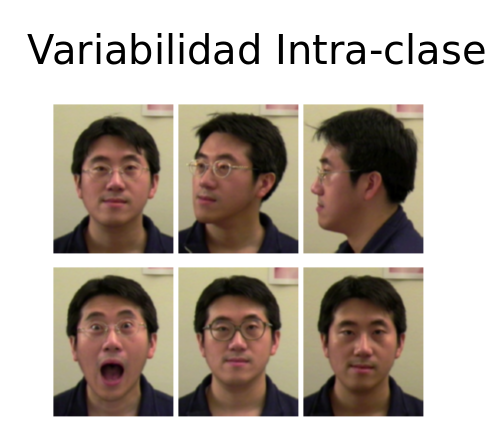
\includegraphics{./Images/ICVariability.png}
\caption{alt text}
\end{figure}

    \begin{figure}[htbp]
\centering
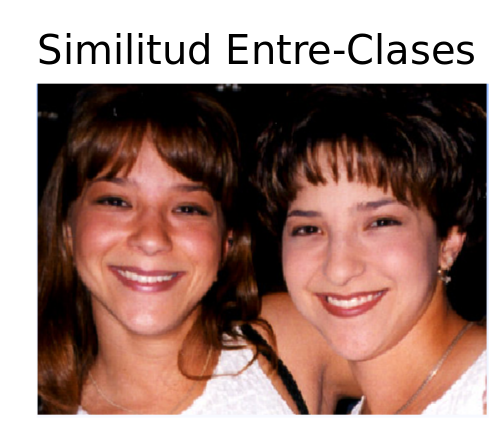
\includegraphics{./Images/ICSimilarity.png}
\caption{alt text}
\end{figure}

    \subparagraph{** Diseño de la etapa de aprendizaje
**}\label{diseuxf1o-de-la-etapa-de-aprendizaje}

    Cuando nos enfrentamos al problema de aprendizaje de máquina debemos
responder a tres preguntas fundamentales:

Cuál es el \textbf{modelo} que vamos a usar teniendo en cuenta el
problema a resolver, es decir la estructura que tiene el conjunto de
datos. Es importante tener en cuenta que todo modelo tiene parámetros
que se deben ajustar para que pueda adaptarse (aprender), el problema
particular que deseamos abordar.

Cuál es el \textbf{criterio} de ajuste del modelo que vamos a usar. Es
decir determinar qué es lo que queremos que haga el modelo con respecto
al conjunto de muestras de entrenamiento y expresarlo a través de una
función matemática.

Cuál es y cómo funciona el \textbf{algoritmo} que encuentra los
parámetros del modelo de acuerdo al criterio escogido. En la mayoría de
los casos la ejecución del criterio de entrenamiento implica un
procedimiento de maximización (o minimización) de la función criterio.
Por consiguiente en esta etapa necesitamos aplicar un algoritmo que
pueda solucionar el problema de optimización.

Como todo procedimiento de modelado, el aprendizaje de máquina debe
pasar por etapas de verificación y validación que permitan establecer el
correcto funcionamiento del modelo propuesto y cuantificar su desempeño
en términos objetivos.

\begin{center}\rule{0.5\linewidth}{\linethickness}\end{center}

    \subsubsection{** Modelos básicos de aprendizaje
**}\label{modelos-buxe1sicos-de-aprendizaje}

    Vamos a centrarnos por un momento en el problema de regresión. Es casi
seguro que para diferentes problemas hayan tenido que utilizar una
regresión lineal, polinomial y/o múltiple, con el propósito de encontrar
una función que pudiera explicar el comportamiento de un conjunto de
datos. Supongamos que queremos modelar un conjunto de datos empleando
una función polinomial de la forma:

\subsubsection{ACA VA UNA FORMULA}\label{aca-va-una-formula}

donde ** \emph{M} ** es el orden del polinomio. ¿Cómo se ajusta
\textbf{w}?

En este caso particular, la función polinomial que hemos escogido
corresponde al modelo que vamos a usar. Necesitamos entonces definir el
criterio por el cual vamos a ajustar los parámetros del modelo, en
particular los pesos wj (El valor de M también requiere ser ajustado,
sin embargo si cambiamos M se está cambiando el órden del polinomio y
por lo tanto el modelo en sí mismo. Más adelante veremos cómo enfrentar
el problema de seleccionar el modelo más adecuado, por ahora supondremos
que el valor de M está dado de manera a prior).

\textbf{El criterio}: La función de error más usada es (** para un mismo
modelo podemos tener diferentes criterios de ajuste**):

\subsubsection{ACA VA UNA FORMULA}\label{aca-va-una-formula-1}

Con esta función de error podemos hallar una \$ f \$ para la cual, la
distancia perpendicular de los puntos \(\mathbf{x}_{i}\) a \$ f \$ sea
mínima.

    \begin{figure}[htbp]
\centering
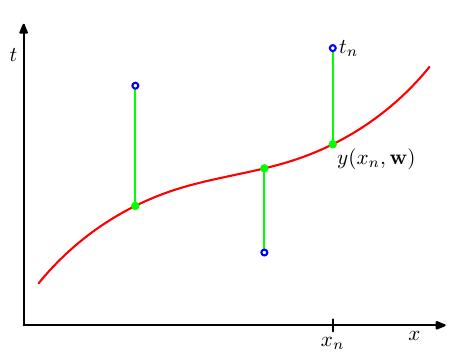
\includegraphics{./Images/Regression.png}
\caption{alt text}
\end{figure}

    Si queremos hayar un \textbf{w} que minimize el error entonces,
derivamos la función de error con respecto a cada uno de los parámetros
\({w}_{j}\):

\section{COLOCAR FORMULA}\label{colocar-formula}

Para efectos de cálculo podemos asumir que el vector \({x}_{i}\)
contiene todas las características de la muestra \$ i \$ y una
característica adicional con valor de 1, que multiplicará al término
independiente \({w}_{0}\).

\section{COLOCAR FORMULA}\label{colocar-formula-1}

Un algoritmo simple que nos permite solucionar el problema de
optimización es el ** Algoritmo ** de Gradiente Descendente. Un problema
de optimización puede tener múltiples formas o algoritmos para
resolverse, cuando el problema de optimización es ** convexo ** podemos
esperar que casi con cualquier método encontremos el valor del parámetro
que hace la función óptima, sin embargo, es posible que el problema de
optimización no sea convexo, en cuyo caso el algoritmo o método de
optimización juega un rol más importante. También es importante tener en
cuenta la velocidad de convergencia del algoritmo o método de
optimización, el costo computacional y el número de parámetros libres.

El algoritmo de gradiente descendente es un algoritmo iterativo que va
actualizando los pesos \({w}_{j}\) en la medida en que estos van
haciendo la función objetivo mínima. La regla de actualización de los
pesos en cada iteración está dada por: \# COLOCAR FORMULA

donde \(η\) se conoce como la tasa de aprendizaje y \(d\) es el número
de variables, independiente de si son polinomiales o no. Para entender
un poco qué hace el algoritmo, consideremos la siguiente \emph{Función
Convexa}

    \begin{Verbatim}[commandchars=\\\{\}]
{\color{incolor}In [{\color{incolor}4}]:} \PY{n}{x} \PY{o}{=} \PY{n}{np}\PY{o}{.}\PY{n}{linspace}\PY{p}{(}\PY{o}{\PYZhy{}}\PY{l+m+mi}{10}\PY{p}{,}\PY{l+m+mi}{10}\PY{p}{,}\PY{l+m+mi}{100}\PY{p}{)}\PY{p}{;}
        \PY{n}{y} \PY{o}{=} \PY{n}{x} \PY{o}{*}\PY{o}{*} \PY{l+m+mi}{2}\PY{p}{;}
        \PY{n}{plt}\PY{o}{.}\PY{n}{plot}\PY{p}{(}\PY{n}{x}\PY{p}{,}\PY{n}{y}\PY{p}{)}
        \PY{n}{plt}\PY{o}{.}\PY{n}{show}\PY{p}{(}\PY{p}{)}
\end{Verbatim}

    \begin{center}
    \adjustimage{max size={0.9\linewidth}{0.9\paperheight}}{output_38_0.png}
    \end{center}
    { \hspace*{\fill} \\}
    

    % Add a bibliography block to the postdoc
    
    
    
    \end{document}
